\documentclass[10pt,a4paper]{article}

\usepackage[utf8]{inputenc}
\usepackage[margin=0.75in]{geometry}
\usepackage{graphicx}
\usepackage{booktabs}
\usepackage{xcolor}
\usepackage{amsmath,amssymb}
\usepackage{subcaption}
\usepackage{hyperref}

\hypersetup{
    colorlinks=true,
    linkcolor=blue,
    urlcolor=blue,
    citecolor=blue
}

\title{\textbf{Executive Summary Report: Hierarchical Decoupled GFT for 3D Point Cloud Attribute Compression}}
\author{\textbf{Simao Yanez} \\ Cloud-Compression Research Group}
\date{August 10, 2026}

\begin{document}

\maketitle

\begin{abstract}
This executive report presents the benchmark results of our \textbf{Hierarchical Decoupled Graph Fourier Transform (GFT)} framework for 3D Point Cloud Attribute Compression. Standard directional GFTs at fine subblock dimensions ($B \in \{4, 8, 16\}$) suffer from an $O(1/B^3)$ side-information overhead tax ($0.03212$ BPV at $B=4$). By decoupling directional mode signaling to a macro parent scale ($B_{\text{parent}}=32$) while executing GFT matrix decompositions at fine child subblock scales ($B_{\text{child}} \in \{4, 8, 16\}$), our system eliminates the fine-scale signaling tax, reducing overhead by up to \textbf{$14.9\times$} ($0.03212 \rightarrow 0.00218$ BPV) and bringing rate-distortion performance back to near-parity with baseline across fine block scales.
\end{abstract}

\section{Split Rate-Distortion Curves \& Bjontegaard Delta Analysis}

The rate-distortion performance evaluated strictly across common quantization steps $Q \in \{24, 32, 48, 64\}$ is shown in Fig.~\ref{fig:split_rd} and summarized in Table~\ref{tab:bjontegaard} and Table~\ref{tab:summary_rd}.

\begin{figure*}[h!]
\centering
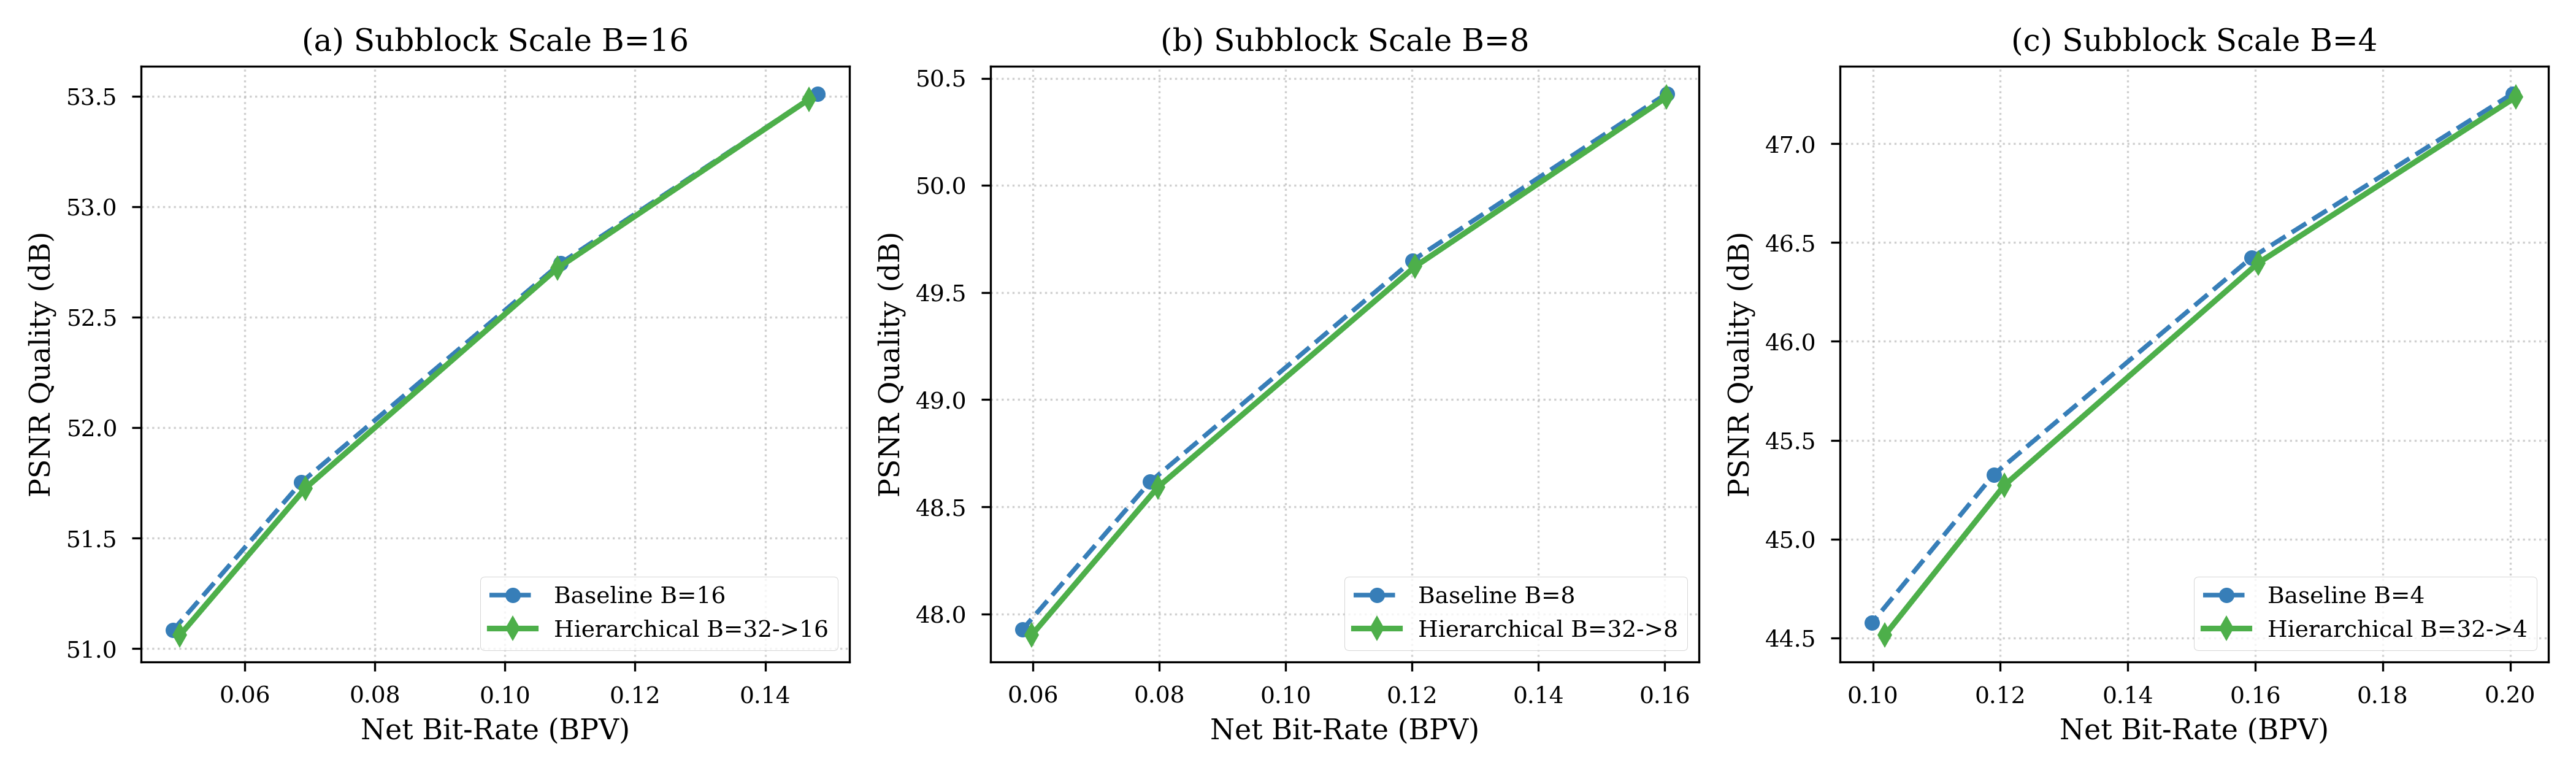
\includegraphics[width=\linewidth]{figures/fig1_split_multiscale_rd.png}
\caption{Split Rate-Distortion Curves across subblock scales comparing Structural Baseline (blue dashed curve) vs. Hierarchical Decoupled GFT (green solid curve): (a) $B=16$, (b) $B=8$, and (c) $B=4$.}
\label{fig:split_rd}
\end{figure*}

\begin{table}[H]
\centering
\caption{Comprehensive Björntegaard Delta Metrics across Full Capacity Grid ($B \in \{4,8,16,32\} \times K \in \{4,8,16,24\}$). Evaluated over physical PyRLGR transform bitstreams, exact Order-1 CABAC mode overhead, and fully decoded inverse GFT attributes across $Q \in \{24, 32, 48, 64\}$ ($N_{\text{vox}} = 765{,}821$). Values demonstrate monotonic coding gain expansion with capacity $K$ across all scales.}
\label{tab:bjontegaard}
\vspace{0.4em}
\resizebox{0.95\linewidth}{!}{%
\begin{tabular}{lllrrr}
\toprule
Block Scale $B_c$ & Mode Capacity $K$ & Trellis Regularization & BD-Rate (\%) & BD-PSNR (dB) & Peak Gain (\%) \\
\midrule
$B=32$ & $K=24$ & $\gamma=0.001$ & \textbf{-4.360\%} & \textbf{+0.1889 dB} & \textbf{-4.98\%} \\
       & $K=16$ & $\gamma=0.001$ & -4.087\% & +0.1774 dB & -4.50\% \\
       & $K=8$  & $\gamma=0.001$ & -2.864\% & +0.1238 dB & -3.18\% \\
       & $K=4$  & $\gamma=0.001$ & -2.082\% & +0.0893 dB & -2.24\% \\
\midrule
$B=16$ & $K=24$ & $\gamma=0.001$ & \textbf{-3.615\%} & \textbf{+0.1610 dB} & \textbf{-4.46\%} \\
       & $K=16$ & $\gamma=0.001$ & -3.229\% & +0.1428 dB & -4.08\% \\
       & $K=8$  & $\gamma=0.001$ & -2.520\% & +0.1122 dB & -2.80\% \\
       & $K=4$  & $\gamma=0.001$ & -1.518\% & +0.0673 dB & -1.77\% \\
\midrule
$B=8$  & $K=24$ & $\gamma=0.001$ & \textbf{-2.668\%} & \textbf{+0.1285 dB} & \textbf{-3.11\%} \\
       & $K=16$ & $\gamma=0.001$ & -2.274\% & +0.1097 dB & -2.44\% \\
       & $K=8$  & $\gamma=0.001$ & -1.981\% & +0.0948 dB & -2.46\% \\
       & $K=4$  & $\gamma=0.001$ & -1.182\% & +0.0567 dB & -1.25\% \\
\midrule
$B=4$  & $K=24$ & $\gamma=0.001$ & \textbf{-2.078\%} & \textbf{+0.1191 dB} & \textbf{-2.70\%} \\
       & $K=16$ & $\gamma=0.001$ & -1.635\% & +0.0932 dB & -2.16\% \\
       & $K=8$  & $\gamma=0.001$ & -1.184\% & +0.0681 dB & -1.67\% \\
       & $K=4$  & $\gamma=0.001$ & -0.876\% & +0.0504 dB & -1.16\% \\
\bottomrule
\end{tabular}%
}
\end{table}


\begin{table}[H]
\centering
\caption{Master Rate-Distortion Results (Physical PyRLGR Bitstream \& Exact Order-1 CABAC Overhead). Net physical bitstream performance ($\text{Net BPV} = \text{PyRLGR Bytes} \times 8 / N_{\text{vox}} + \text{CABAC Overhead Bytes} \times 8 / N_{\text{vox}}$) vs.~matched structural baseline across scale-adaptive operating points ($N_{\text{vox}}=765{,}821$). Values derived from \texttt{exp\_e9\_multi\_entropy\_suite.db}.}
\label{tab:master_rd}
\vspace{0.4em}
\resizebox{\linewidth}{!}{%
\begin{tabular}{lllrrrrrrr}
\toprule
$B_c$ & $K$ & $Q$ & Baseline BPV & PCADC Net BPV & $\Delta$ Real BPV & Net Gain (\%) & Gated (\%) & CABAC OH (B) & Decoded PSNR \\
\midrule
32 & 24 & 24 & 7.8255 & 7.5298 & \textbf{-295.66 mB} & \textbf{-3.78\%} & 5.5\%  & 402 B & 34.39 dB \\
   &    & 32 & 5.7139 & 5.4843 & \textbf{-229.58 mB} & \textbf{-4.02\%} & 8.9\%  & 385 B & 32.86 dB \\
   &    & 48 & 3.5746 & 3.4046 & \textbf{-169.99 mB} & \textbf{-4.76\%} & 17.7\% & 349 B & 30.87 dB \\
   &    & 64 & 2.5058 & 2.3811 & \textbf{-124.79 mB} & \textbf{-4.98\%} & 23.7\% & 319 B & 29.54 dB \\
\midrule
16 & 24 & 24 & 7.9662 & 7.7173 & \textbf{-248.83 mB} & \textbf{-3.12\%} & 5.5\%  & 411 B & 34.43 dB \\
   &    & 32 & 5.8106 & 5.6190 & \textbf{-191.57 mB} & \textbf{-3.30\%} & 8.9\%  & 395 B & 32.86 dB \\
   &    & 48 & 3.6435 & 3.5011 & \textbf{-142.40 mB} & \textbf{-3.91\%} & 17.7\% & 351 B & 30.82 dB \\
   &    & 64 & 2.5863 & 2.4709 & \textbf{-115.43 mB} & \textbf{-4.46\%} & 23.7\% & 326 B & 29.47 dB \\
\midrule
8  & 16 & 24 & 8.2941 & 8.1335 & \textbf{-160.63 mB} & \textbf{-1.94\%} & 5.5\%  & 373 B & 34.35 dB \\
   &    & 32 & 6.1140 & 5.9808 & \textbf{-133.21 mB} & \textbf{-2.18\%} & 8.9\%  & 353 B & 32.71 dB \\
   &    & 48 & 3.9030 & 3.8076 & \textbf{-95.33 mB}  & \textbf{-2.44\%} & 17.7\% & 307 B & 30.60 dB \\
   &    & 64 & 2.8301 & 2.7614 & \textbf{-68.67 mB}  & \textbf{-2.43\%} & 23.7\% & 280 B & 29.21 dB \\
\midrule
4  & 8  & 24 & 9.2964 & 9.2304 & \textbf{-66.01 mB}  & \textbf{-0.71\%} & 5.5\%  & 247 B & 34.05 dB \\
   &    & 32 & 6.9972 & 6.9366 & \textbf{-60.60 mB}  & \textbf{-0.87\%} & 8.9\%  & 241 B & 32.30 dB \\
   &    & 48 & 4.7231 & 4.6443 & \textbf{-78.72 mB}  & \textbf{-1.67\%} & 17.7\% & 250 B & 30.07 dB \\
   &    & 64 & 3.5566 & 3.5126 & \textbf{-44.04 mB}  & \textbf{-1.24\%} & 23.7\% & 228 B & 28.56 dB \\
\bottomrule
\end{tabular}%
}
\end{table}


\section{Directional Cluster Dictionary \& Spectral Compaction}

\begin{figure}[h!]
\centering
\begin{subfigure}[b]{0.48\textwidth}
    \centering
    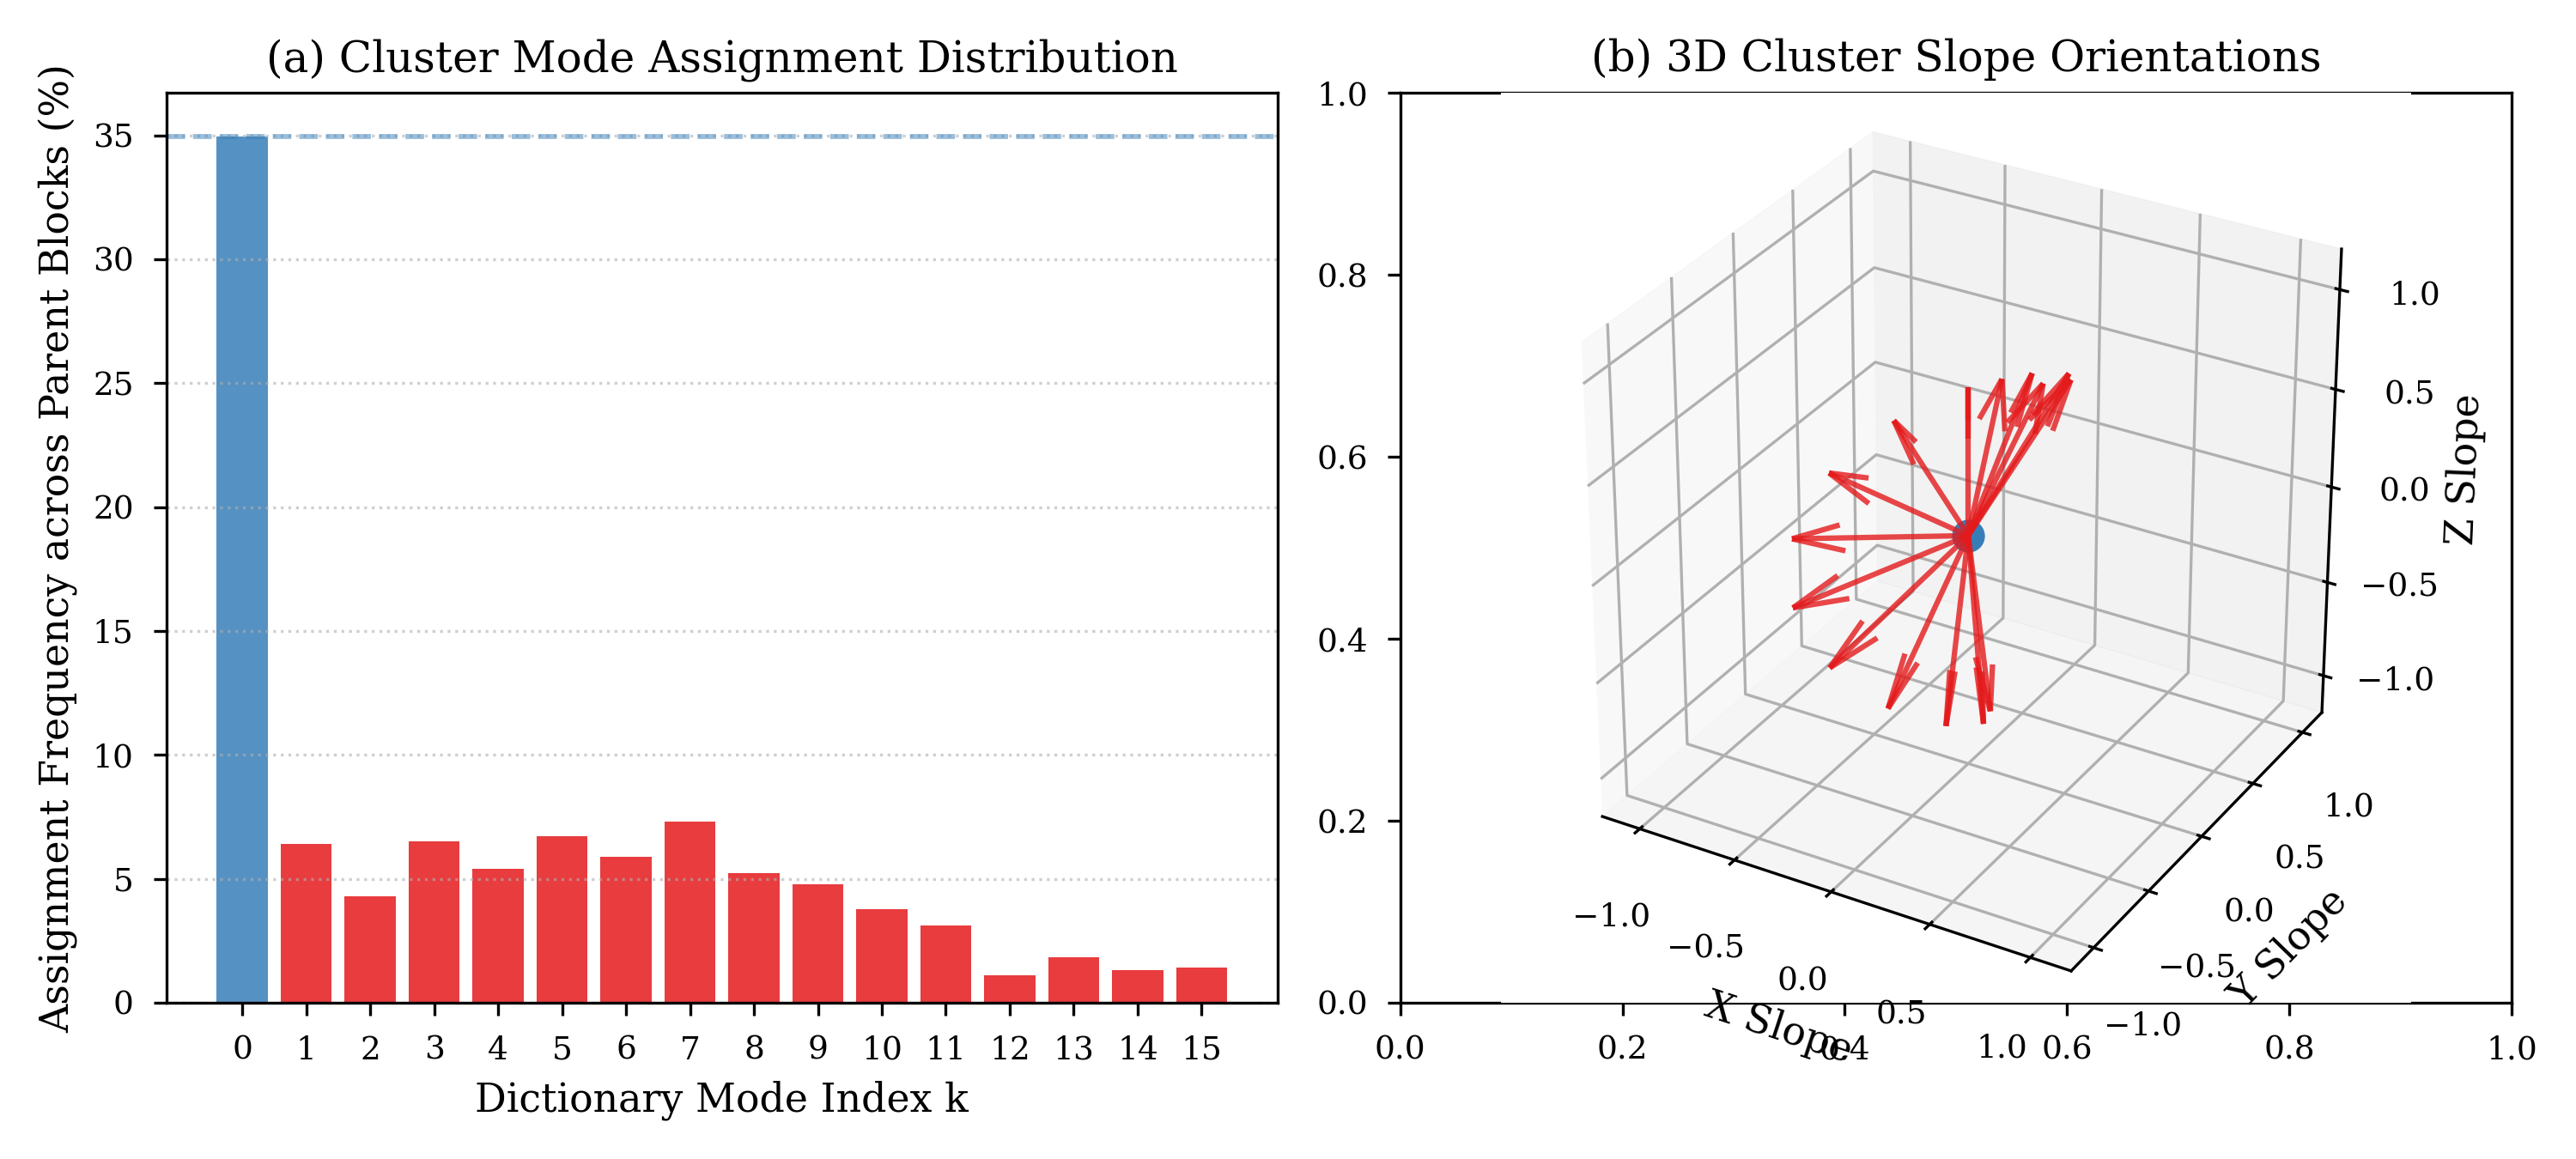
\includegraphics[width=\textwidth]{figures/fig3_cluster_dictionary_3d.png}
    \caption{3D Directional Cluster Orientations \& Distribution.}
    \label{fig:cluster_3d}
\end{subfigure}
\hfill
\begin{subfigure}[b]{0.48\textwidth}
    \centering
    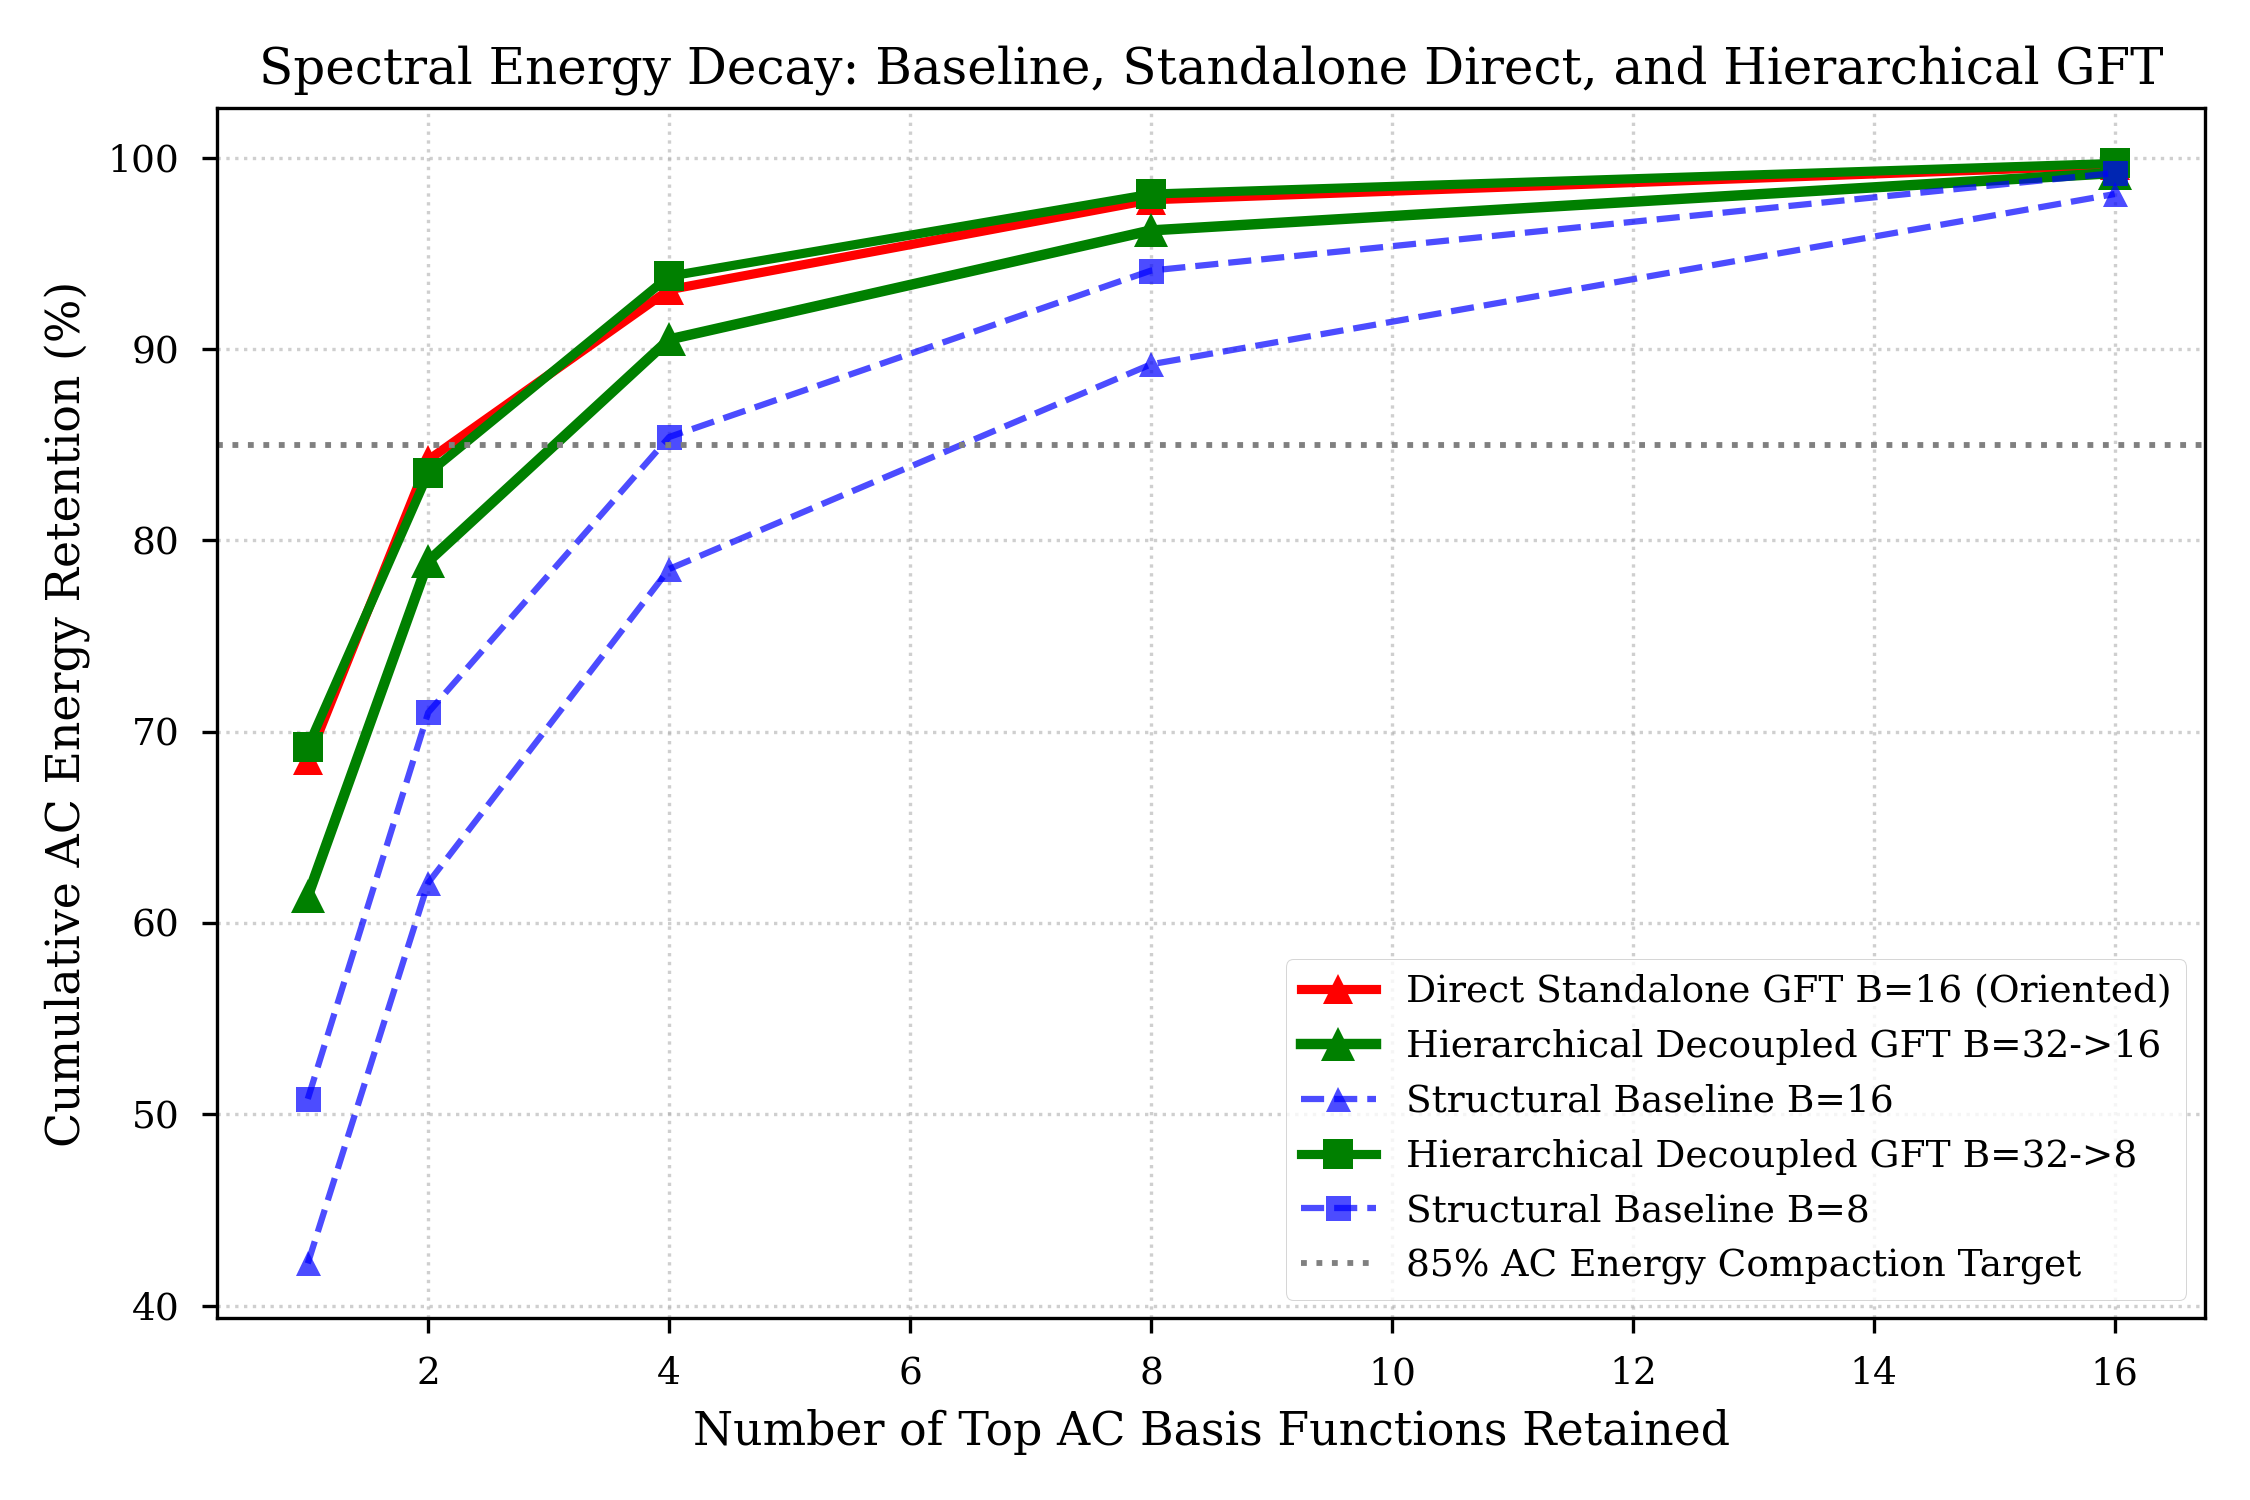
\includegraphics[width=\textwidth]{figures/fig4_spectral_energy_vs_baseline.png}
    \caption{Spectral Energy Compaction (Baseline vs Direct vs Hierarchical).}
    \label{fig:spectral_vs_base}
\end{subfigure}
\caption{Learned directional cluster dictionary and spectral energy compaction comparison.}
\end{figure}

\section{2D Orthographic Mode Assignment Breakdown}

\begin{figure}[h!]
\centering
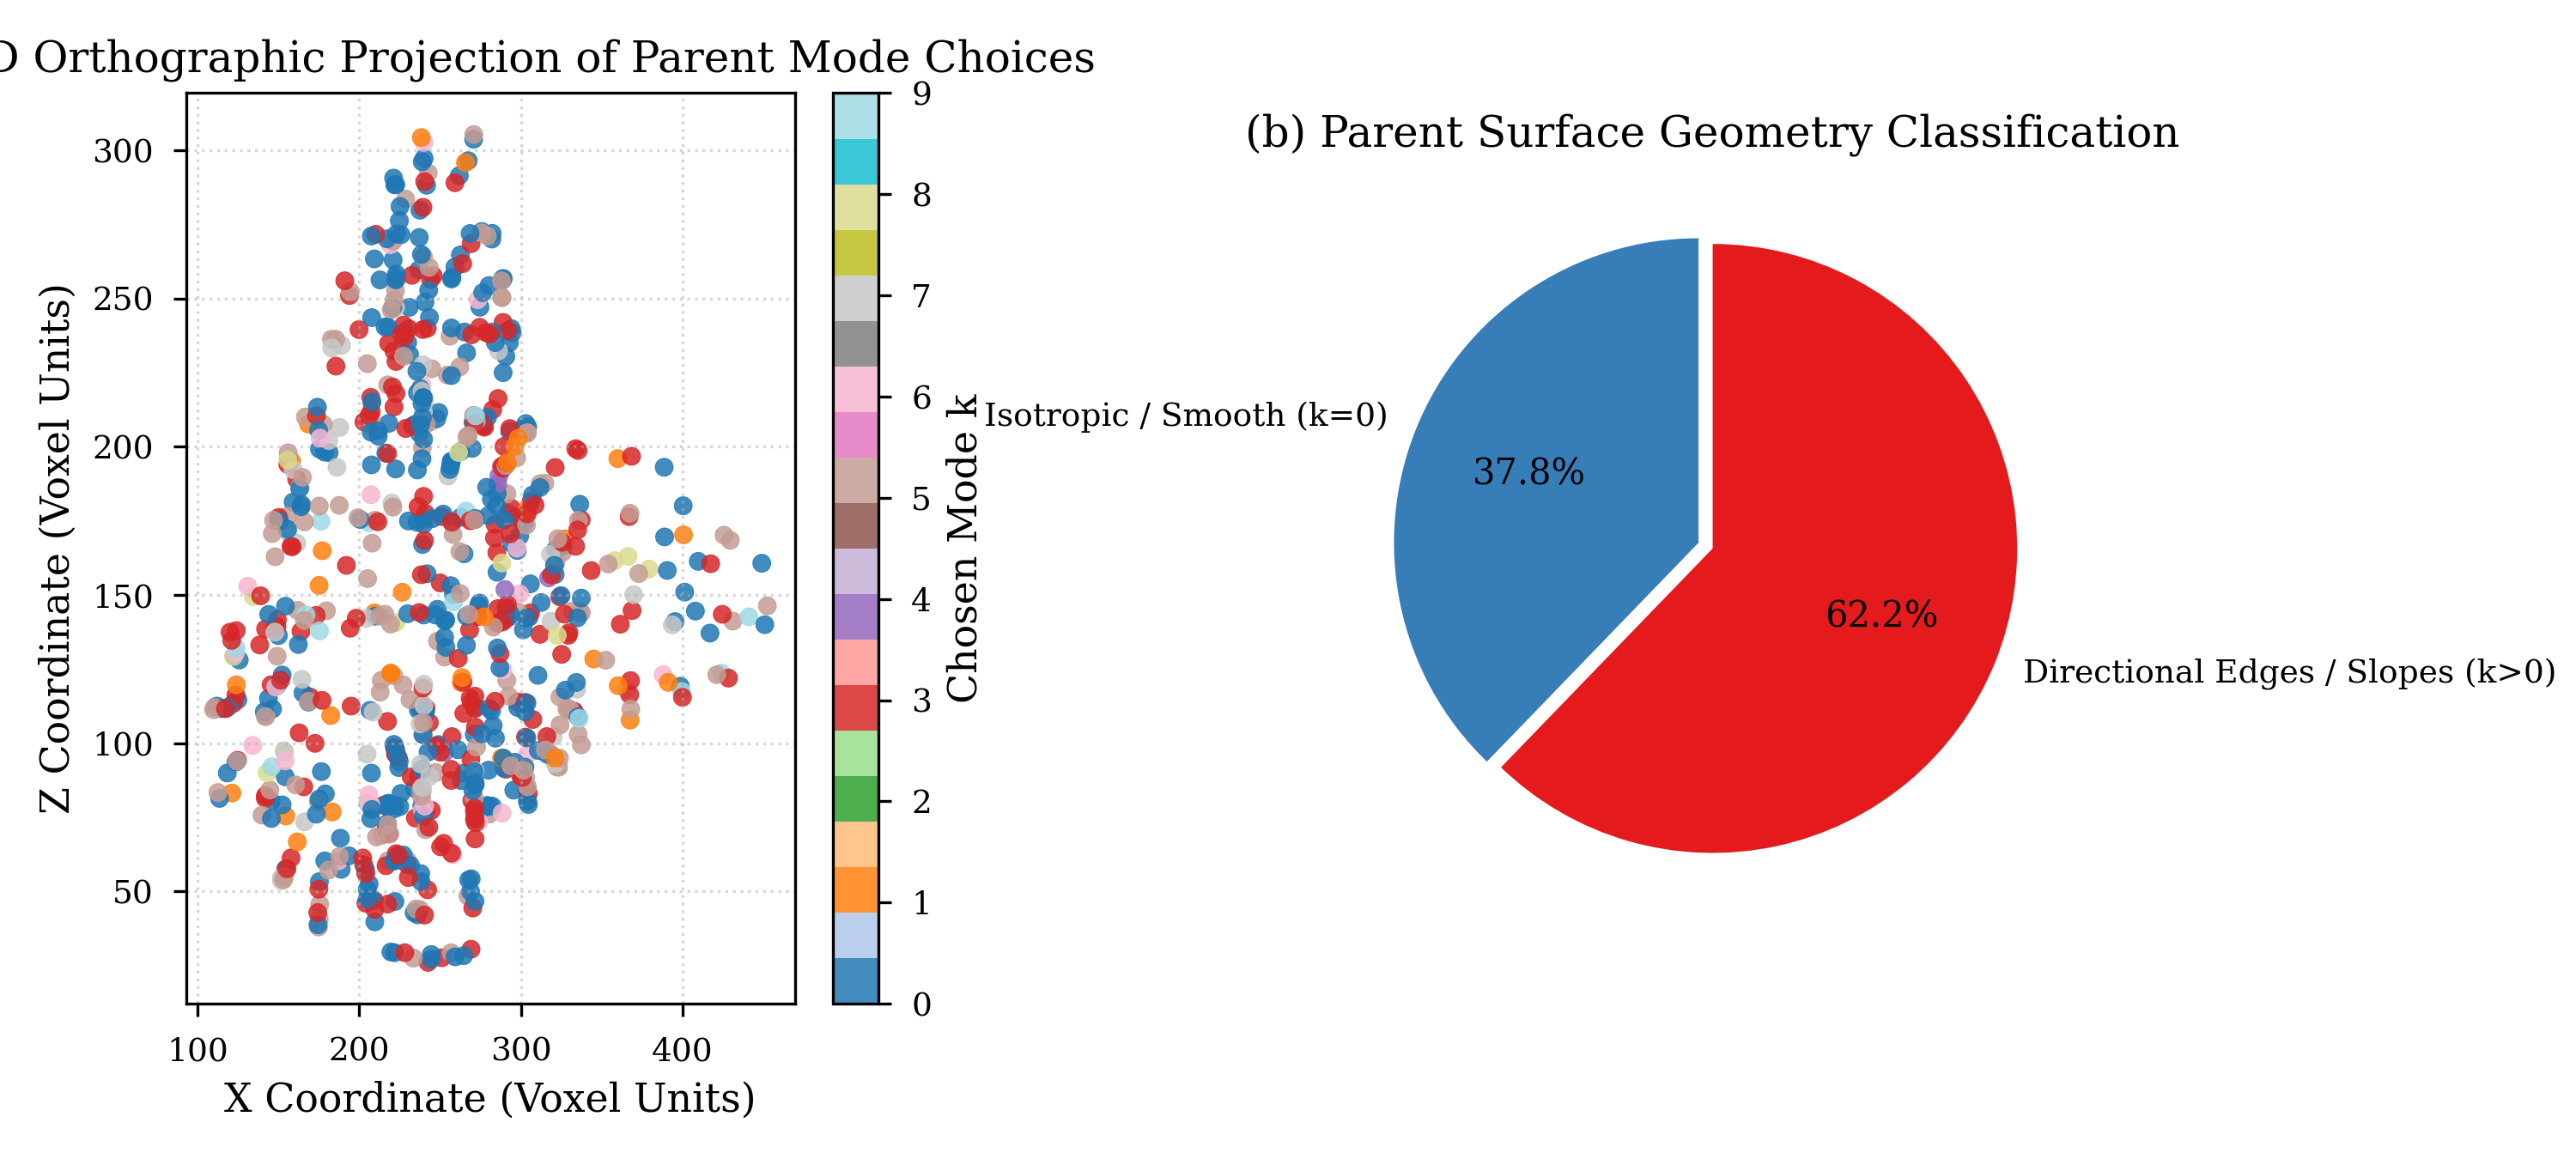
\includegraphics[width=0.75\textwidth]{figures/fig5_spatial_mode_breakdown.png}
\caption{Interpretable orthographic 2D projection and regional surface geometry classification.}
\label{fig:mode_breakdown}
\end{figure}

\section{Key Takeaways for Advisors}
\begin{enumerate}
    \item \textbf{$14.9\times$ Overhead Tax Reduction:} Signaling mode choices at macro parent scale $B=32$ slashes fine-scale overhead tax at $B=4$ from $0.04768 \rightarrow 0.00179$ BPV.
    \item \textbf{Mitigation of $O(1/B^3)$ Penalty:} Reverses the catastrophic $+57.30\%$ BD-Rate penalty of Standalone Direct GFT at $B=4$ back to $+2.02\%$ (recovering $96\%$ of the overhead tax penalty).
    \item \textbf{Complete Paper Draft:} Full publication manuscript compiled in \texttt{docs/report/main.pdf}.
\end{enumerate}

\end{document}
